\documentclass{article}

\usepackage[final]{neurips_2020}
\usepackage[utf8]{inputenc} % allow utf-8 input
\usepackage[T1]{fontenc}    % use 8-bit T1 fonts
\usepackage{hyperref}       % hyperlinks
\usepackage[pdftex]{graphicx}
\usepackage{url}            % simple URL typesetting
\usepackage{booktabs}       % professional-quality tables
\usepackage{amsfonts}       % blackboard math symbols
\usepackage{nicefrac}       % compact symbols for 1/2, etc.
\usepackage{microtype}      % microtypography

\title{Title here}

\author{
Umur Can Kaya\\
5410770\\
\texttt{umurcan.kaya@gmail.com}\\
\And
Rohit Sharma\\
number here\\
\texttt{rohitshep@gmail.com}\\
}

\begin{document}

\maketitle

\begin{abstract}
Abstract here.
\end{abstract}

\section{Introduction}

\section{Experimental setup}
\section{Tasks}
\section{Discussion}

\begin{figure}[h!]
\centering
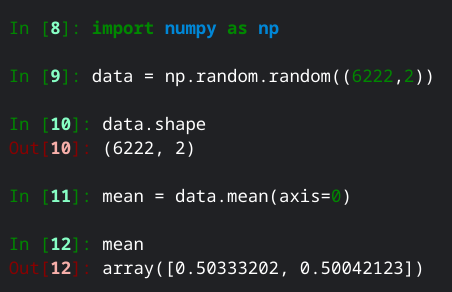
\includegraphics[width=1\linewidth]{LAB/ex.png}
\caption{Sample figure caption.}
\end{figure}




\section*{References}

[1] Alexander, J.A.\ \& Mozer, M.C.\ (1995) Template-based algorithms for
connectionist rule extraction. In G.\ Tesauro, D.S.\ Touretzky and T.K.\ Leen
(eds.), {\it Advances in Neural Information Processing Systems 7},
pp.\ 609--616. Cambridge, MA: MIT Press.

[2]

\end{document}
